\chapter{Syntax-Driven Verification} % compare to CFG-driven
% TODO: mention that recursion is not covered here

\section{Introduction}
While the methodology presented in the previous chapter
for verifying memory preservation works well, it is not ideal.
\index{memory!preservation}
The need to manually formulate regions
and the amount of work required for developing invariants
\index{Floyd!invariant}
reduces potential scalability.
\index{scalability}

To build on the work from the previous chapter,
this chapter introduces the concept of \emph{\acp{fmuc}}
generated by untrusted, informal tools.
\Acp{fmuc} consist of two main components:
theorems on \hyperref[ch:memory]{memory usage} and \emph{proof ingredients}.
\index{memory!usage}
\index{proof!ingredients}
The proof ingredients are assumptions on memory layout,
control flow information, and invariants
generated to reduce the amount of work required from end users.
Information on how these certificates are generated can be found in \cref{se:fmuc_gen}.
This includes the algorithm for control flow information extraction
as well as how symbolic execution is used
to produce the preconditions and proof ingredients.
\index{symbolic execution}

Once generation is complete, the certificate and the original assembly
\index{certificate}
can then be loaded into an interactive theorem prover.
In the theorem prover,
\index{theorem!prover}
minimal user input is required for discharging \iac{fmuc}'s lemmas and theorems
via the proof ingredients and customized proof strategies.
\index{proof!ingredient}
\index{proof!strategy}
A simple example demonstrating usage along with 
further information on the structure of \acp{fmuc} can be found in \cref{se:fmuc_ex}.

After going into further detail on \acp{fmuc} verification in \cref{se:fmuc_ver},
\cref{se:syntax_example} provides an example to illustrate the generation
and verification process.
On its own, that example could theoretically overwrite its own return address
due to its pointer arguments, causing \ac{cfi} issues.
The associated \ac{fmuc} provides preconditions to prevent such cases
along with a formal proof of return address preservation under those conditions. 

Following the more full example in \cref{se:syntax_example} is a full case study
on the Xen Project hypervisor~\citep{chisnall2008definitive} in \cref{se:xen}.
\index{Xen}
Unlike the HermitCore work in \cref{se:cfg_application},
\index{HermitCore}
no modifications were made to the Xen build process
and the basic utility \texttt{objdump} was used for disassembly.
In total, \acp{fmuc} were generated and proofs discharged in Isabelle
for 251 Xen functions.
Minimal user interaction was required;
on average, only \num{85} lines of additional proof were needed
for every \num{1000} assembly instructions verified.
In total, the \num{12252} assembly instructions
were verified with only \num{1047} manual proof lines added,
all of which were simple reuses of established proof methods.
The majority of added lines of proof involved guiding loop invariant application.
\index{loop!invariant}

\section{Overview of \acsp*{fmuc}}\label{se:fmuc_ex}
\Cref{fig:fmuc} provides an example of \iac{fmuc}.
\Acp{fmuc} are produced from assembly code,
which may be generated by a disassembler such \texttt{objdump}, IDA\fturl{https://www.hex-rays.com/products/ida/index.shtml},
Ghidra's decompiler\fturl{https://ghidra-sre.org/}, or Capstone~\citep{capstone},
or generated directly by a compiler when source code is available.
Each function specified for verification receives \iac{fmuc};
those that are not included in the verification effort,
including system calls and functions from dynamic libraries,
can be treated as black boxes, the usage of which is described in \cref{sse:fmuc_comp}.

\begin{figure*}
  \centering
  \lstset{frame=none, numbers=none}
  \begin{subfigure}{.51\linewidth}
    \begin{lstlisting}[language=C, gobble=6]
      int main(int argc, char** argv) {
          return argv[argc - 1][0];
      }
    \end{lstlisting}
    \caption{Source code}\label{fig:example-src}
  \end{subfigure}
  \begin{subfigure}{.48\linewidth}
    \begin{lstlisting}[style=x64, basicstyle=\footnotesize\ttfamily, gobble=6]
      4f0: movsxd rdi, edi
      4f3: mov rax, qword ptr [rsi+rdi*8-8]
      4f8: movsx eax, byte ptr [rax]
      4fb: ret
    \end{lstlisting}
    \caption{Compiled assembly}\label{fig:example-asm}
  \end{subfigure}
  \begin{subfigure}{\linewidth}
    \centering
    \begin{align*}
      \text{\bfseries Theorem: } & \var{MRR}\Longrightarrow\htriple*{P}{f}{Q}{M} \\
      \text{\bfseries Proof: } & \ldots
    \end{align*}
    where
    \begin{align*}
      f &\equiv\ABB~\Block{4f0}{4fb} \\
      P &\equiv\mathrip=
      \mathtt{4f0}\wedge\mathrsp=\rspo\wedge\ldots\wedge\readmem{\rspo}{8}=\retaddr \\
      Q &\equiv\begin{multlined}[t]
        \mathrip=\retaddr\wedge\mathrsp=\rspo+8\wedge\ldots\wedge \\
        \langle 31,0\rangle\mathrax=\sextend(\readmem{\readmem{\rsio+\sextend(\langle 31,0\rangle\rdio)*8-8}{8}}{1})
      \end{multlined} \\
      M &\equiv\begin{cases}
        \region{\rspo}{8} & \hypertarget{m:a}{(a)} \\
        \region{\rsio+\sextend(\langle 31,0\rangle\rdio)*8-8}{8}
        & \hypertarget{m:b}{(b)} \\
        \region{\readmem{\rsio+\sextend(\langle 31,0\rangle\rdio)*8-8}{8}}{1}
        & \hypertarget{m:c}{(c)}
      \end{cases} \\
      \var{MRR} &\equiv\begin{aligned}
        \not\bowtie &= \{\} \\
        \sqsubseteq &= \{\}
      \end{aligned}
    \end{align*}
    \caption{\Acl*{fmuc}\footnote{%
      $\sextend$ indicates sign extension,
      $\langle h,l\rangle w$ indicates taking bits $l$ through $h$ of word $w$,
      and $\readmem{a}{n}$ indicates reading $n$ bytes of memory
      starting at address $a$.
    }}\label{fig:fmuc-thm}
  \end{subfigure}
  \caption{Example \ac{fmuc}}\label{fig:fmuc}
\end{figure*}

The small program shown in \cref{fig:example-src} provides a simple example
for \ac{fmuc} explanation. This one-function program
returns the numeric value of the first character of its last command-line argument.
When compiled to assembly (x86-64 using the System V \ac{abi}),
the program will resemble the code depicted in \cref{fig:example-asm}.
In this assembly code,
\lstinline|argc| maps to the register \inlineasm{edi},
which is the low 32 bits of the 64-bit register \inlineasm{rdi},
and \lstinline|argv| maps to \inlineasm{rsi}.
After sign-extending \inlineasm{edi} to fill \inlineasm{rdi},
that value and the other argument are used to calculate
an address, stored in the register \inlineasm{rax},
from which a one-byte value is read.
That value sign extended and stored in the lower 32 bits of \inlineasm{rax},
\inlineasm{eax}.

As stated in the introduction to this chapter, \iac{fmuc} consists of two main parts:
a theorem on memory usage and its associated proof ingredients,
\index{memory!usage}
\index{proof!ingredient}
the two of which are used in a theorem prover to prove the theorem.
The \ac{fmuc} for the associated example can be seen in \cref{fig:fmuc-thm}.

The theorem consists of a Hoare triple as defined in \cref{def:usage}.
\index{Hoare!triple}
One set of proof ingredients,
the \acp{mrr} required to ensure successful proof completion (detailed below),
are included as assumptions on the theorem.
The control flow ingredient,
represented as the \ac{scf} variable~$f$, is a single basic block for this function
starting at instruction \inlineasm{4f0} and going to instruction \inlineasm{4fb}.
Following that, the precondition~$P$ provides the starting conditions for the function,
which include symbolic variables for initial register values,
storage on the stack of the address to jump to after function execution,
and the address of the instruction to start from
(stored in the instruction pointer register, \inlineasm{rip}).
Last of the traditional Hoare triple components is the postcondition~$Q$,
which indicates completion of function execution
by showing that the instruction pointer is now set to the address to return to,
the stack pointer \inlineasm{rsp} has been updated with an increment of eight,
and the return value register, \inlineasm{rax},
contains the value \lstinline|argv[argc - 1][0]|.
All additional callee-saved registers are shown to retain their initial values as well.
\index{register!callee-saved}

Following the traditional Hoare triple elements is the memory region set,~$M$.
\index{Hoare!triple}
For the function under consideration, this set consists of three regions.
The eight-byte location of the return address
on the stack frame (\hyperlink{m:a}{$a$}),
the location of the pointer \lstinline|argv[argc - 1]| (\hyperlink{m:b}{$b$}),
and the first element of the array pointed to by that pointer (\hyperlink{m:c}{$c$}).
Without additional assumptions, those regions may \emph{alias};
\index{memory!aliasing}
they may overlap or even be the same.
While that is not a problem for this specific example,
as none of the regions are written to,
in cases where writes do occur
aliasing can result in writes to regions that are not considered by symbolic execution.
This can result in requirements for significant effort on the part of proof engineers,
greatly reducing automation.
To avoid such issues, the \ac{fmuc} generation methodology
produces the aforementioned \acp{mrr} proof ingredient,
\index{proof!ingredient}
the production of which is detailed in \cref{sse:mem_reg}.
\Acp{mrr} express which pairs of regions are not separate ($\not\bowtie$)
\index{memory!region!separation}
as well as which regions are enclosed within one another ($\sqsubseteq$).
\index{memory!region!enclosure}

The \ac{fmuc} for a function as a whole is broken down by Hoare rules
\index{Hoare!rule}
as described in \cref{se:hoare_rules} to the level of basic blocks,
each of which gets its own \ac{fmuc} of sorts.
The generation of these per-block \acp{fmuc} involves generation of per-block
pre- and postconditions as well; these conditions are treated as invariants.
\index{Floyd!invariant}
Stronger invariants can lead to a tighter approximation of memory usage
\index{memory!usage}
(remember, the memory usage here is an overapproximation).

With the \acp{fmuc} as generated, their theorems and proof ingredients all considered,
minimal effort is required in the vast majority of cases to complete the proofs.
The main exception is functions containing loops.
For functions that do have loops, as well as for any other cases where proof completion
\index{loop}
is not automatic, Isabelle/HOL proof strategies as documented in \cref{se:fmuc_ver}
\index{Isabelle/HOL}
provide assistance in completing the proofs efficiently.

\section{\acs*{fmuc} Generation}\label{se:fmuc_gen}
\begin{figure*}
  \centering
  \begin{tikzpicture}[>=stealth, gnode/.style={draw, rounded corners, text centered}]
    \graph[grow right=2.8cm]{
      Assembly[gnode] ->[dashed]
      "Control Flow Graph"[gnode, text width=1.4cm] ->["\ref{sse:cfg_extract}"]
      "Syntactic Control Flow"[gnode, text width=1.7cm] ->["\ref{sse:mem_reg}"]
      "Memory Regions and \acsp*{mrr}"[gnode, text width=1.5cm] ->["\ref{sse:inv_gen}"]
      Invariants[gnode] ->[dashed] Certificate[gnode];
    };
  \end{tikzpicture}
  \caption{FMUC Overview}\label{fig:overview}
\end{figure*}

The general procedure for generating \acp{fmuc}, laid out in \cref{fig:overview},
can be broken up into three main parts.
The first part involves control flow extraction from assembly using \iac{cfg} analysis
similar to angr's CFGFast~\citep{shoshitaishvili2016state},
\index{angr!CFGFast}
ultimately producing \iac{scf} (details of which are presented
in \cref{sse:cfg_extract}).
Afterwards, per-basic block symbolic execution,
\index{basic block}
\index{symbolic execution}
as detailed in \cref{ch:symbolic_execution},
is utilized to generate the set of memory regions
\index{memory!region}
read and written by the function in question.
To eliminate duplicates and produce \acp{mrr}
showing which regions overlap or are enclosed or separate,
\index{memory!region!enclosure}
\index{memory!region!separation}
the region sets are fed to the \ac{smt} solver Z3~\citep{de2008z3}
as described in \cref{sse:mem_reg}.
% TODO: may not need the second subsection as we describe symbolic execution elsewhere
Symbolic execution is also used in the process of generating
the pre- and postconditions for each basic block as seen in \cref{sse:inv_gen},
which are involved in the process of per-block verification
and Hoare rule application.
\index{Hoare!rule}

With the exception of \ac{mrr} generation,
none of the steps in this procedure are included in the \ac{tcb}.
The process of verifying the generated \ac{fmuc} (see \cref{se:fmuc_ver})
will fail if there are issues in control flow extraction,
\ac{scf} generation, informal symbolic execution, or invariant generation.
\Ac{mrr} generation is an exception
because the \acp{mrr} are formulated as assumptions,
and thus inconsistent \acp{mrr} will result in vacuous proofs.
This is why the methodology relies on Z3 for \ac{mrr} generation;
\index{Z3}
using a known-reliable tool greatly reduces the possibility of issues.

\subsection{Control Flow Extraction}\label{sse:cfg_extract}
As described in \cref{se:hoare2,se:hoare_rules},
in order to apply \iac{vcg} that utilizes Hoare rules to verify a Hoare triple,
\index{Hoare!rule}
\index{Hoare!triple}
there must be some syntactic structure to apply those rules to.
This chapter uses a syntactic representation of control flow called \ac{scf}
for that purpose.
\Ac{scf} expresses assembly programs as a combination of basic blocks, branches, loops,
and function calls.
The following grammar provides a description of \ac{scf}
from the perspective of the Haskell code
\index{Haskell}
(the formulation in Isabelle/HOL is slightly different).
\index{Isabelle/HOL}
Each basic block is represented by the polymorphic type~$\beta$,%
\nomenclature{$\beta$}{Type of basic blocks}
while branching conditions are represented using the polymorphic type~$\phi$.%
\nomenclature{$\phi$}{Type of branching conditions}
\begin{bnf}
  \bnfprod*{scf}{
    \bnfpn{scf}\bnfsp\bnfts{;}\bnfsp\bnfpn{scf}
    \bnfor\bnfts{Block}\bnfsp\bnftd{$\beta$}
    \bnfor\bnfts{Skip}
    \bnfor\bnfts{Continue}
    \bnfor\bnfts{Break}\bnfsp\bnfpn{br}
  } \\
  \bnfmore{
    \bnfor\bnfts{If}\bnfsp\bnftd{$\phi$}
      \bnfsp\bnfts{Then}\bnfsp\bnfpn{scf}
      \bnfsp\bnfts{Else}\bnfsp\bnfpn{scf}
      \bnfsp\bnfts{Fi}
    \bnfor\bnfts{Loop}\bnfsp\bnfpn{scf}\bnfsp\bnfts{Pool}\bnfsp\bnfpn{res}
  } \\
  \bnfprod{br}{
    \bnftd{ID}\bnfor\bnfes
  } \\
  \bnfprod{res}{
    \bnfts{Resume}\bnfsp\bnfts{\{(}\bnftd{ID}\bnfts{,}\bnfpn{scf}\bnfts{),}\bnfsk\bnfts{\}}
    \bnfor\bnfes
  }
\end{bnf}
Loops in this formulation have no exit condition;
\index{loop}
instead, they rely on having one or more internal \texttt{Break} statements,
\index{loop!break}
which may have an identifier to indicate how the loop was exited, for termination.
\texttt{Continue}s function the same as in C,
\index{loop!continue}
causing loop execution to skip to the next iteration.
For loops that have multiple exit points,
\texttt{Resume} statements provide different code to execute
based on which exit was taken as indicated by the \texttt{Break} identifier.

Notably, the above data structure does not explicitly contain
control flow statements such as \texttt{goto} or \texttt{throw/catch}
as those statements are not necessary for assembly-level analysis.
A non-indirect \texttt{goto} is simply an unconditional jump,
which is just another singular edge in the \ac{cfg},
and structured exception handling as used in C++ is generally represented
by library-supplied and compiler-generated function calls.

There are a couple of important restrictions on the control flow extraction approach
presented in this section,
the more severe of which is the lack of support for indirect branching.
Handling indirect branching requires a more in-depth \ac{cfg} analysis
than that done here,
as the targets of indirect branches cannot necessarily be determined statically.
As all other forms of conditional branching have only two branches,
the above data structure uses the if-then-else statement to represent all forms of
conditional branching.
The lesser restriction on control flow extraction is that the algorithm is not optimal
due to the just-mentioned fact that if-then-else statements
are the only method of representing multiple branches
as well as the restrictions on loop structure.
This is elaborated on in \cref{sse:code_dup},
which provides an example where one basic block is repeated twice
in the generated \ac{scf}.

\subsubsection{Syntactic Control Flow in Isabelle/HOL}
There are some modifications to the \acp{scf} when loaded into Isabelle/HOL
\index{Isabelle/HOL}
due to how the Hoare rules in \cref{se:hoare_rules} are applied.
In that representation, there are no \texttt{Break}s or \texttt{Continue}s;
any occurrences of such statements are translated to \texttt{Skip}.
This does mean that programs that cannot be easily transformed
such that that translation does not modify the overall semantics
are not easily handled in this framework.
However, none of functions encountered in the case study presented in \cref{se:xen}
had that issue, so it does not appear to be a significant drawback.

Additionally, loops in the Isabelle/HOL syntax do rely on a explicit exit condition.
\index{loop}
This condition is simply the precondition of the entry block of the loop
as generated using the methodology in \cref{sse:inv_gen}.

Finally, to properly handle function calls in the Isabelle/HOL syntax,
analyzed \acp{cfg} are preprocessed prior to performing extraction
to isolate \inlineasm{call} instructions into their own basic blocks.
\index{basic block}
These single-instruction blocks are then translated into \texttt{Call}~$f$ entries
in the Isabelle/HOL \ac{scf}, where~$f$ is the textual label of the function called.

\subsection{Extraction Algorithm}
\begin{algorithm}
  \caption{Control flow extraction}\label{algo:cf}
  \begin{algorithmic}[1]
    \Require{A subgraph $\var{sg}=(B,E,L)$ and its entry block}
    \Ensure{Result is syntactic control flow of type $\scf(B,E_F)$}
    \Function{cfgToScf}{$\var{sg},\var{entry}$}
      \State $\var{sccs}\gets\Call{sccs}{\var{sg}}$
        \Comment{Implicit argument to subcalls, along with $\var{entry}$}
        \label{line:scc1}
      \If{$\abs{\var{sccs}}=1$}\nomenclature{$\abs\cdot$}{Indicates size of~$\cdot$}
          \Comment{Only one \acs*{scc} present, may be a recursive loop}
        \State $\var{sccs}\gets\Call{sccs}{\var{sg}-\text{edges to }\var{entry}}$
        \label{line:scc2}
      \EndIf
      \State \letin{[\var{entry},b_1,\dotsc,b_k]}
      {\var{entry}\ll b_1\ll\dotsb\ll b_k\ll\bot}%
      \nomenclature{$\ll$}{Indicates post-dominance; in this dissertation,
        it is restricted to immediate post-dominance}
      \label{line:ipdoms}
      \State\Return $\Call{stmts}{\var{entry},b_1,\true};
      \Call{stmts}{b_1,b_2,\false};\dotsb;
      \Call{stmts}{b_k,\bot,\false}$
    \EndFunction
    \Function{stmts}{$b,b_j,\var{first}$}
      \State\Return $\begin{cases}
        \ASkip & \text{if }b=b_j \\
        \AContinue & \text{if }b=\var{entry}\wedge\neg\var{first} \\
        \ABreak(\ID(\Call{pre}{b})) & \text{if }\var{sccs}(b)=\bot \\
        \ABB b & \text{if }\abs{\Call{post}{b}}=0 \\
        \AWhile~\ABB b~\AOd & \text{if }\Call{post}{b}=\{b\}
      \end{cases}$\label{line:prepost}
      \State \letin{b'}{b\ll b'}\Comment{$b'$ may be~$b_j$}
      \State $a_0\gets\begin{cases}
        \Call{loop}{b,b'} & \text{if }\abs{\var{sccs}(b)}>1 \\
        \ABB b & \text{if }\abs{\Call{post}{b}}=1 \\
        \Call{singleLoop}{b,b_e} & \text{if }\Call{post}{b}=\{b,b_e\} \\
        \Call{ite}{b,b_0,b_1,b'} & \text{if }\Call{post}{b}=\{b_0,b_1\}
      \end{cases}$\label{line:post}
      \State $a_1\gets\begin{cases}
        \Call{stmts}{b',b_j,\false} & \text{if }b'\neq\bot \\
        \ASkip & \text{otherwise}
      \end{cases}$
      \State\Return $a_0;a_1$
    \EndFunction
    \Function{singleLoop}{$b,b_e$}
      \State\Return $\AWhile~\ABB b;
      \AIf~L(b,b_e)~\AThen~\ABreak(\ID b)~\AElse~\ASkip~\AFi~\AOd$
    \EndFunction
    \Function{ite}{$b,b_0,b_1,b'$}
        \State\Return $\ABB b;\AIf~L(b,b_0)~\AThen~
        \Call{stmts}{b_0,b',\false}~\AElse~\Call{stmts}{b_1,v',\false}~\AFi$
    \EndFunction
    \Function{loop}{$b,b'$}\label{line:loop}
      \State $\var{scc}\gets\var{sccs}(b)$
      \State $a\gets\Call{cfgToScf}{\var{scc},b}$
      \State $\var{resumes}\gets\{(i,a')\mid
      \exists b_0~b_e\cdot i=\ID b_0\wedge
      \Call{exit}{b_0,b_e,\var{scc}}\wedge a'=\Call{stmts}{b_e,b',\false}\}$
      \State\Return $\AWhile~a~\AOd~\AWhileResume\var{resumes}$
    \EndFunction
  \end{algorithmic}
\end{algorithm}

\Cref{algo:cf} presents the methodology for control flow extraction
used in this chapter.
The first input is a (sub-)\ac{cfg}, an edge-labeled graph $(B,E,L)$.
$B$ is the set of all vertices in the graph, the basic blocks.%
\nomenclature{$B$}{Concrete type of basic blocks}
\index{basic block}
These blocks are represented by their start and end addresses.
Following on from~$B$, $E:B\rightarrow\powerset(B)$%
\nomenclature{$\powerset(\cdot)$}{Indicates power set of $\cdot$}
indicates the edges originating from each block
and $L:B\times B\rightarrow E_F$ is a labeling function.
The label type,~$E_F$, consists of logical expressions over flags.%
\nomenclature{$E_F$}{Label type, logical expressions over flags}
Thus, the control flow extraction algorithm
produces \iac{scf} with $\beta=B$ and $\phi=E_F$.

The algorithm, \textsc{cfgToScf}, operates recursively, starting with the full \ac{cfg}
of the function under consideration.
It decomposes the \ac{cfg} into a sequence of syntactic statements
using the subfunction \textsc{stmts}, which also operates recursively.
If any potentially non-trivial loops are encountered
in the execution of \textsc{stmts},
\textsc{cfgToScf} is again called with the bodies of those loops as subgraphs.

The following paragraphs elaborate on the notation and functions
used in the text of the algorithm.
Functions \textsc{pre} and \textsc{post} (\cref{line:prepost,line:post})
respectively return the parent and child blocks of the block that is their argument.
% \bot explained in Nomenclature, no need to do so here
The helper function \textsc{sccs} (\cref{line:scc1,line:scc2})
returns the \acp{scc} of the subgraph supplied to it,
the subgraphs of that subgraph that are all strongly connected.
A \emph{strongly connected} graph is one
\index{strongly connected}
where each of its vertices is reachable from every other vertex.
\Iac{scc} is trivial if it consists of only one element and is not a loop.
The \acp{scc} are stored as a partial surjection
\index{surjection}
from blocks to their corresponding \acp{scc}.
If block~$b$ is not in subgraph~$\var{sg}$,
then $\textsc{sccs}(\var{sg})(b)$ returns~$\bot$.
Function $\textsc{exit}(b_0,b_1,\var{sg})$ checks if~$b_1$ is an \emph{exit child}
\index{exit child}
of~$b_0$; that is, it checks if~$b_1$ is a child of $b_0$,
that~$b_0$ is in $\var{sg}$, and that~$b_1$ is not.

Next, notation $b_0\ll b_1$ expresses that block~$b_1$
\emph{immediately post-dominates}~$b_0$.
\index{dominance!post!immediate}
This means two things:
\begin{enumerate}
  \item $b_1$ strictly post-dominates~$b_0$:
  all paths to an exit block of the \ac{cfg} that start at~$b_0$
  must go through~$b_1$ and $b_0\neq b_1$.
  \item $b_1$ does not strictly post-dominate
  any other strict post-dominators of~$b_0$.
\end{enumerate}
The paths involved in post-dominance calculation include those in loops,
so if a \ac{cfg} contains a block~$b_0$
that loops back on itself and has one child~$b_1$,
then~$b_1$ is still considered the immediate post-dominator of~$b_0$.
\index{dominance!post!immediate}
Only exit blocks lack immediate post-dominators, a situation denoted as $b\ll\bot$.
As every block has at most one immediate post-dominator
and no other block in its path will have the same one,
there exists a unique chain of blocks formed by the immediate post-dominance relation
for every starting block that leads to an exit.

Now that the terminology and notation not elsewhere defined is out of the way,
the behavior of \textsc{cfgToScf} itself can be discussed.
It starts by computing the \acp{scc} of the supplied subgraph,~$\var{sg}$.
If~$\var{sg}$ consists of a single non-trivial \ac{scc}, it is a loop,
\index{loop}
a situation that only happens when the function is recursive.
\index{recursion}
Otherwise, the \ac{cfg} either has multiple \acp{scc} or one trivial \ac{scc}.
As the recursive loop situation cannot be handled in that exact form,
it is broken by removing all back edges to the entry block
and recomputing the \acp{scc}.
The immediate post-dominance chain of blocks in the subgraph
that follow from the entry block is then produced (\cref{line:ipdoms})
and used to construct a sequence of \acl{scf} statements
extracted from every immediate post-dominance pair,
ending with a statement extracted from the exit block.

Statement extraction occurs in the \textsc{stmts} function.
It is also recursive, operating from block~$b$ to a \emph{joint} block,~$b_j$,
\index{basic block!joint}
and has multiple base cases.
The first is when execution has reached the joint block,
in which case the function produces \texttt{Skip}.
Alternatively, if~$b$ is the entry block for the current subgraph
but this is not the first time \textsc{stmts} has been called
for the current invocation of \textsc{cfgToScf},
then the \ac{cfg} has jumped back to the start of a loop
and the result should be \texttt{Continue}.
\index{loop!continue}
There is also the possibility of the current block
not being present in the current set of \ac{scc} and thus not in the current subgraph,
indicating that a loop has been exited.
In that case, a \texttt{Break} is generated
\index{loop!break}
and annotated with the ID of the parent block, the one that caused the exit.
The next two cases to consider are based on the children of the current block~$b$.
If it has no children, then the result is a single \texttt{Block}
with~$b$ as its argument.
In contrast, if its only child is itself then it is a simple, one-block infinite loop
and is returned as such.

In the remaining cases,
the algorithm produces one or more sequences of \ac{scf} components;
the components from~$b$ to its immediate post-dominator~$b'$ (stored in~$a_0$)
\index{dominance!post!immediate}
sequenced with those from~$b'$ to~$b_j$ ($a_1$, which may be \texttt{Skip} if,
for whatever reason,~$b$ has no immediate post-dominator).
If there are multiple \acp{scc} in the current mapping,
a non-trivial loop is present and requires loop analysis between~$b$ and~$b'$,
performed by \textsc{loop}.
Next, if~$b$ only has one child, it can be mapped to a simple \texttt{Block}.
The two remaining cases involve~$b$ having two children,
meaning there is a conditional jump.
If one of~$b$'s children is itself and the other is some block~$b_c$,
then it forms a single-block loop that exits to~$b_c$.
Otherwise,~$b$ and its two children produce an if-then-else statement.

Loop extraction in \textsc{loop} (\cref{line:loop}) requires two steps.
\index{loop!extraction}
First, the body of the loop is extracted using a (recursive) call to \textsc{cfgToScf}.
Second, the \ac{scf} components between every exit child of the current \ac{scc}
and the joint block~$b'$ are stored in a set, associated with the corresponding
\index{basic block!joint}
exit child's ID, and supplied to the loop's \texttt{Resume} statement.
This ensures that the control flow is properly configured
for all exit points of the loop.

\begin{example}
  \Cref{fig:ex_cf} provides an example of \ac{scf} extracted from \iac{cfg}.
  At the first call of \textsc{cfgToScf},
  the post-dominator relation is $0\ll 6\ll\bot$
  \index{dominance!post}
  and thus $\textsc{stmts}(0,6,1)$ and $\textsc{stmts}(6,\bot,0)$ are computed.
  For the first call to \textsc{stmts},
  term~$a_0$ becomes an if statement computed by $\textsc{ite}(0,1,7,6)$
  and term~$a_1$ is computed by $\textsc{stmts}(6,6,0)$.
  The computed if statement has two branches,
  with this example considering the branch where~$f_0$ holds.
  Extraction for that branch computes $\textsc{stmts}(1,6,0)$.
  As $1\ll 5$, that call results in $a_0=\textsc{loop}(1,5)$
  and $a_1=\textsc{stmts}(5,6,0)$.
  The loop body in~$a_0$ is extracted from subgraph $\{1,2\}$,
  \index{loop}
  while the paths from~$4$ to~$5$ and~$3$ to~$5$ continue after the loop.
  Term~$a_1$ is simply $\ABB 5$.
\end{example}

\begin{figure*}
  \hspace*{\fill}
  \subcaptionbox{Example \ac*{cfg}\label{fig:ex_cf_cfg}}{
    \begin{tikzpicture}[->, >=stealth, node distance=0.75cm]
      \node[draw=none] (0) {0};
      \node[draw=none] (1) [below=of 0] {1};
      \node[draw=none] (2) [below=of 1]{2};
      \node[draw=none] (3) [below=of 2]{3};
      \node[draw=none] (4) [left=of 3, xshift=0.5cm, yshift=0.5cm]{4};
      \node[draw=none] (5) [below=of 3]{5};
      \node[draw=none] (6) [below=of 5, xshift=0.5cm, yshift=0.5cm]{6};
      \node[draw=none] (7) [right=of 1]{7};
      \node[draw=none] (8) [right=of 3, xshift=0.5cm, yshift=0.5cm]{8};
      \node[draw=none] (9) [right=of 5]{9};
      
      \path (0) edge node[left]{$f_0$} (1);
      \draw[rounded corners=2mm] (0) -| node[above, xshift=0.4cm, yshift=-0.9cm]{$\neg f_0$} (7);
      \path (1) edge [bend left] node[right]{$f_1$} (2);
      \draw[rounded corners=2mm] (1) -| node[left, yshift=-1.3cm]{$\neg f_1$} (4);
      \path (2) edge [bend left] node[left, xshift=0.1cm]{$f_2$} (1);
      \path (2) edge node[right]{$\neg f_2$} (3);
      \path (3) edge node[right]{} (5);
      \draw[rounded corners=2mm] (4) |- (5);
      \path (5) edge node[right]{} (6);
      \draw[rounded corners=2mm] (7) -| node[right, yshift=-1.3cm]{$\neg f_7$} (8);
      \path (7) edge node[left, yshift=-1cm]{$f_7$} (9);
      \draw[rounded corners=2mm] (8) |- (9);
      \path (9) edge node[right]{} (6);
    \end{tikzpicture}
  }
  \hfill
  \subcaptionbox{Syntactic Control Flow}{
    \(\begin{array}{l}
      \ABB 0; \\
      \AIf~f_0~\AThen \\
      \ind{2ex}\AWhile \\
      \ind{4ex}\ABB 1; \\
      \ind{4ex}\AIf~f_1~\AThen \\
      \ind{6ex}\ABB 2;~\AIf~f_2~\AThen~\AContinue~\AElse~\ABreak 2~\AFi \\
      \ind{4ex}\AElse~\ABreak~1~\AFi \\
      \ind{2ex}\AOd~\AWhileResume\{(2,\ABB 3), (1,\ABB 4)\} \\
      \ind{2ex}\ABB 5 \\
      \AElse \\
      \ind{2ex}\ABB 7; \\
      \ind{2ex}\AIf~f_7~\AThen~\ASkip~\AElse~\ABB 8~\AFi; \\
      \ind{2ex}\ABB~9 \\
      \AFi; \\
      \ABB 6
    \end{array}\)
  }
  \hspace*{\fill}
  \caption{Example of control flow extraction}\label{fig:ex_cf}
\end{figure*}

\subsection{Extraction Algorithm Analysis}
The control flow extraction algorithm presented above
does not necessarily need any formal reasoning as it is not included in the \ac{tcb}
for this chapter.
However, showing that it \emph{terminates} and is \emph{sound} still has worth.
\index{termination}
\index{soundness}
Thus, a proof of correctness for a modified version
of the syntactic control flow data structure,
excluding if-then-else statements and using direct recursion,
\index{recursion}
was formulated in Isabelle/HOL.
\index{Isabelle/HOL}
As a complement,
this subsection presents informal proofs of termination and soundness
for the extraction algorithm.
It also provides an example where the algorithm is not optimal
due to syntactic duplication caused by the limited branch representation.

\subsubsection{Termination}
Showing termination is slightly tricky as the two main functions involved,
\textsc{cfgToScf} and \text{stmts}, are mutually recursive.
\index{recursion!mutual}
However, if a separate strictly-decreasing \emph{measure}
\index{recursion!measure}
can be shown for each function, termination as a whole will then follow.

\begin{proof}
  The measure for \textsc{cfgToScf} is based on its subgraph argument.
  Every subcall will have a strictly smaller number of blocks in its supplied subgraph.
  This can be seen as, if the entire graph is strongly connected
  such that all of its blocks are in one single \ac{scc},
  the algorithm will remove the back edges to the entry block
  and then recompute the \acp{scc}.
  By the definition of strong connection,
  \index{strongly connected}
  that operation ensures there will be two or more smaller \acp{scc}
  for the modified graph.
  As any further calls to \textsc{cfgToScf} will take one of those \acp{scc},
  the reduction in blocks is guaranteed and thus so is \text{cfgToScf}'s termination.
  
  Termination of function \texttt{stmts} instead relies on the fact
  that it is always called under the condition $b\ll b_j$ (except when $b=b_j$).
  That precondition ensures that all paths starting from~$b$ that reach the exit
  must necessarily go through~$b_j$.
  As the function recursively explores the children of~$b$,
  having base cases when there are no more blocks to explore,
  the only possibility for non-termination is a loop occurring before~$b_j$.
  That loop may be either a single-block loop or \iac{scc} with more than one element.
  Neither case results in a direct recursive call of \texttt{stmts},
  thus ensuring termination.
\end{proof}

\subsubsection{Soundness}
The proof of soundness for control flow extraction,
showing that the semantics of \iac{cfg} is equivalent to those of \iac{scf},
is roughly as follows.
\begin{proof}
  This informal proof is expressed using potentially-infinite \emph{execution paths}.
  \index{execution!path}
  As an example, one possible execution path for \cref{fig:ex_cf_cfg}
  is $[0, 7, 9, 6]$.
  The semantics of both \iac{cfg} and a term of type $\scf(B,E_F)$
  can be expressed in terms of such execution paths.
  With~$\Pi$ as the type of execution paths,%
  \nomenclature{$\Pi$}{Type of execution paths}
  $\sem_\mathrm{CFG}:B\rightarrow\powerset(\Pi)$ and $\sem_\mathrm{SCF}:\scf(B,E_F)\rightarrow\powerset(\Pi)$ respectively denote
  \ac{cfg} and \ac{scf} semantics.
  The first function takes \iac{cfg} entry point as input
  and ``runs'' the \ac{cfg} from there.
  The second function takes \iac{scf} as input and ``runs'' it.
  Soundness for function \textsc{cfgToScf} is defined as follows:
  \begin{equation*}
    \forall b\cdot\sem_{CFG}(b)=\sem_\mathrm{SCF}(\textsc{cfgToScf}(\var{cfg},b)).
  \end{equation*}
    Meanwhile, for \textsc{stmts}, the definition is:
  \begin{equation*}
    \forall b~b_j~f\cdot b\ll b_j\longrightarrow\takeuntil(\sem_\mathrm{CFG}(b),b_j)
    =\sem_\mathrm{SCF}(\textsc{stmts}(b,b_j,f)).
  \end{equation*}
  Function $\takeuntil$ takes a set of execution paths
  and returns all the path prefixes
  that come before the first occurrence of joint block~$b_j$.

  The proof itself is done by induction over \textsc{cfgToScf},
  \index{induction}
  which produces a mutual induction scheme due to the mutual recursion involved.
  
  The first step considers the \emph{sequentialization}
  of terms $\textsc{stmts}(b_i,b_{i+1},t)$.
  The induction hypothesis provides soundness for each of those terms.
  As $b_0\ll b_1\ll\dotsb$, the semantics of the \ac{cfg}
  produces execution paths that can be split up into multiple fragments,
  $[\pi^0_0, \pi^0_1,\dotsc]$.
  Each fragment~$\pi^0_i$ starts at~$b_i$
  and consists of the prefix of the execution path
  up until the first occurrence of $b_{i+1}$.
  The result returned by \textsc{cfgToScf} is of the form~$c_0;c_1;\dotso$,
  which also consists of fragments in the form $[\pi^1_0,\pi^1_1,\dotsc]$.
  The induction hypothesis shows that for all~$i$, $\pi^0_i=\pi^1_i$.
  
  The next step considers the soundness of \textsc{stmts},
  \index{soundness}
  which is largely straightforward.
  In the trivial case where $b=b_j$, both semantics are~$[]$, the empty path.
  That is,
  \begin{equation*}
    \takeuntil(\sem_\mathrm{CFG}(b),b)=\sem_\mathrm{SCF}(\textsc{stmts}(b,b,f))=
    \sem_\mathrm{SCF}(\ASkip)=\{[]\}.
  \end{equation*}
  The case for loops is more intricate.
  \index{loop}
  The semantics of a loop with entry point~$b_e$
  \index{loop!entry}
  is defined as the set of paths from~$b_e$ that can be split into three subpaths.
  The first subpath consists of the loop iterations,
  a list of any number of paths from~$b_e$ to~$b_e$.
  The second subpath is a path from~$b_e$ to an exit.
  The third subpath is a \emph{resume}, a path from an exit to the joint~$b_j$.
  The algorithm produces a loop only if~$b_e$ is in a non-trivial \ac{scc}.
  Under that condition, the set of paths between~$b_e$ and the joint
  is exactly equal to the semantics of a loop.
\end{proof}

\subsubsection{Code Duplication}\label{sse:code_dup}
The algorithm is not optimal in terms of generated \ac{scf} size
as basic blocks may be duplicated.
There are two situations where basic block duplication occurs,
one less common and one more common.
The less common situation is when \iac{scc} has multiple entry blocks.
This corresponds to a loop having multiple entry points,
which can occur in situations that involve less-structured control flow,
such as a C program that jumps into a loop using \texttt{goto}.
Such situations are relatively uncommon, even in optimized code.
If it does happen, the entire loop must be duplicated.
The more common situation, by contrast, involves complex conditional branching
that can occur even without loops.
\Cref{fig:ex_nonopt} shows a small example of branching control flow
that results in $\ABB 3$ being duplicated.
That block could itself be an even more complicated subgraph,
possibly leading to exponential code duplication.
\begin{figure}
  \hspace*{\fill}
  \subcaptionbox{\acs*{cfg}}{
    \begin{tikzpicture}[>=stealth, ->, node distance=0.75cm]
      \node[draw=none] (0) {0};
      \node[draw=none] (1) [right=of 0] {1};
      \node[draw=none] (2) [right=of 1] {2};
      \node[draw=none] (3) [right=of 2] {3};
      \node[draw=none] (4) [right=of 3] {4};

      \path (0) edge node[below]{$f_0$} (1);
      \path (0) edge [bend left] node[above]{$\neg f_0$} (4);
      \path (1) edge node[above]{$f_1$} (2);
      \path (1) edge [bend right] node[below]{$\neg f_1$} (3);
      \path (2) edge node[above]{$f_2$} (3);
      \path (2) edge [bend right] node[below]{$\neg f_2$} (4);
      \path (3) edge (4);
    \end{tikzpicture}
  }
  \hfill
  \subcaptionbox{\acs*{scf}}{
    \(\begin{array}{l}
      \ABB 0; \\
      \AIf~f_0~\AThen~\ABB 1; \\
      \ind{2ex}\AIf~f_1~\AThen~\ABB 2; \\
      \ind{4ex}\AIf~f_2~\AThen~\ABB 3 \\
      \ind{4ex}\AElse~\ASkip~\AFi \\
      \ind{2ex}\AElse~\ABB 3~\AFi \\
      \AElse~\ASkip~\AFi; \\
      \ABB 4
    \end{array}\)
  }
  \hspace*{\fill}
  \caption{Example of code duplication}\label{fig:ex_nonopt}
\end{figure}

\subsection{Memory Region and Region Relation Generation}\label{sse:mem_reg}
This process primarily relies on unverified symbolic execution in the generation code.
\index{symbolic execution}

% TODO

\subsection{Invariant Generation}\label{sse:inv_gen}




\section{\acs*{fmuc} Verification}\label{se:fmuc_ver}
\subsection{Composition}\label{sse:fmuc_comp}

\section{Examples}\label{se:syntax_example}

\section{Application: Xen Project}\label{se:xen}
The Xen Project~\citep{chisnall2008definitive}
\index{Xen}
is a mature, widely-used \ac{vmm}, also known as a \emph{hypervisor}.
\index{hypervisor}
Hypervisors provide a method of managing multiple
\acp{vm} (called domains in the Xen documentation) on a physical host.
\index{domain}
%Xen has support for hardware-assisted virtualization, referred to as \acp{hvm}. % Relevant because of QEMU

The Xen hypervisor is a suitable case study because of its security relevance
\index{Xen}
and its complex build process involving real production code.
Security is a significant issue in environments where hypervisors are used,
such as the \ac{aec2}, Rackspace Cloud, and many other cloud service providers.
For example, when one or more hosts support guest domains
for any number of distinct users,
ensuring isolation of the domains is important.

The Xen build process produces multiple binaries
that contain functions not present in the Xen source itself.
This is due to the inclusion of external static libraries and programs.
Xen version 4.12 was compiled with \ac{gcc} 8.2 via the standard Xen build process.
This build process uses various optimization levels, ranging from \texttt{O1} to \texttt{O3}.
The version of \texttt{objdump} used to disassemble the compiled binaries
was 2.31.1.
\index{objdump}

The verification effort presented here
covered three of the binaries produced by the Xen build process:
\lstinline|xenstore|, \lstinline|xen-cpuid|, and \lstinline|qemu-img-xen|.
The \lstinline|xenstore| binary is involved in the functionality of
XenStore\fturl{https://wiki.xen.org/wiki/XenStore},
a hierarchical data structure shared amongst all Xen domains.
This sharing allows for the possibility of inter-domain communication,
though in general XenStore is intended for simple configuration information.
A smaller program than \lstinline|xenstore|, \lstinline|xen-cpuid|
provides functionality similar to that of the
\lstinline|cpuid| utility\fturl{https://linux.die.net/man/1/cpuid}.
This utility queries the underlying processors
and displays information about the features they support.
Such functionality is important for Xen
as it supports migrating domains
between processors with different variants of the same \ac{isa}~\citep{cpuid-masking}.
The third binary used, \lstinline|qemu-img-xen|,
consists of over three hundred functions
that are not present in the Xen source code.
It provides some of the functionality of \ac{qemu}.
\Ac{qemu} is a free, open-source emulator\fturl{https://www.qemu.org/}.
\index{emulator}
Xen uses it to emulate \acp{dm}, which provide interfaces for hardware storage.

\begin{table*}
  \sisetup{table-format=5.0, table-number-alignment=right}
  \centering
  \begin{tabular}{lrSSS}
    \toprule
    Binaries & Function Count & {Instruction Count} & Loops & {Manual Lines of Proof} \\
    \midrule
    \lstinline|xenstore| & 2/6 & 100 & 0 & 6 \\
    \lstinline|xen-cpuid| & 2/3 & 210 & 2 & 39 \\
    \lstinline|qemu-img-xen| & 247/343 & 11942 & 64 & 1002 \\
    Total & 251/352 & 12252 & 65 & 1047 \\
    \bottomrule
  \end{tabular}
  \caption{Verified Xen Functions}\label{func-counts}
\end{table*}
\begin{figure*}
  \centering
  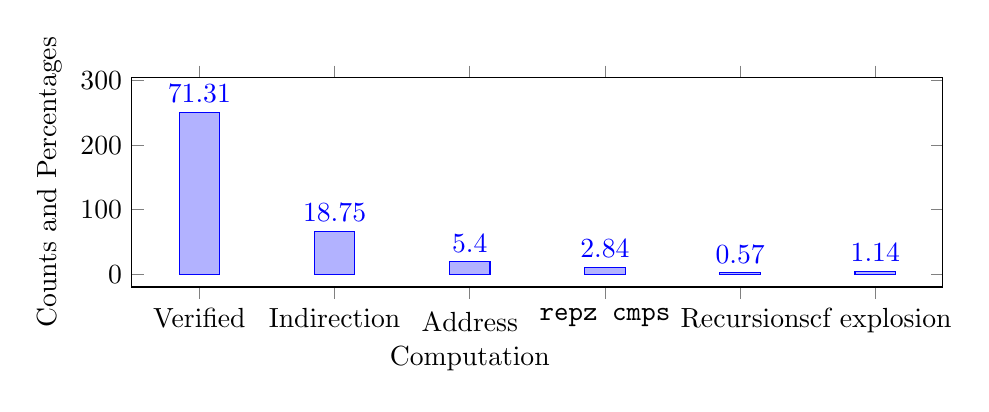
\begin{tikzpicture}
    \begin{axis}[
      width=0.98\linewidth,
      height=0.35\linewidth,
      ybar,
      ylabel=Counts and Percentages,
      bar width=0.3,
      nodes near coords, % causes build failure when combined with symbolic x coords
      point meta=y/3.52, % can't get \% shown right
      enlarge y limits={value=0.2, upper},
      ymin=-20,
      xticklabels={
        Verified,
        Indirection,
        \begin{tabular}{c}Address\\Computation\end{tabular},
        \texttt{repz cmps},
        Recursion,
        \acs{scf} explosion
      },
      xtick=data
    ]
    \addplot coordinates {
      (0, 251)
      (1, 66)
      (2, 19)
      (3, 10)
      (4, 2)
      (5, 4)
    };
    \end{axis}
  \end{tikzpicture}
  \caption{Analzyed Xen Functions Compared to Unverified Features}
  \label{fig:unverified}
\end{figure*}

This methodology is currently capable of dealing with \xenpercentage\
of the functions present in the aforementioned binaries (see \cref{fig:unverified}).
The supported features include (nested) loops,
subcalls, variable argument lists, jumps into other function bodies,
string instructions with the \texttt{rep} prefix, and \ac{simd} instructions.
There is no particular limit on function size.
The average number of instructions per function analyzed is 49.
Some of the functions analyzed have over 300 instructions and over 100 basic blocks.

There are five categories of features not currently supported.
The first and most common, previously mentioned in \cref{sse:cfg_extract},
is \emph{indirection}, accounting for \SI{19}{\percent}.
\index{indirection}
Indirection involves a call or jump instruction
that loads the target address from a register or memory location
rather than using a static value.
Switch statements and certain uses of \texttt{goto}
are the most common causes of indirect jumps.
Indirect calls generally result from usage of function pointers.
For example, the \lstinline|main| functions of all three verified binaries
used switch statements in loops in the process of parsing command line options.
These statements introduced indirect branches.

The second category involves issues related to generating the \acp{mrr}.
This step requires solving linear arithmetic over symbolically computed addresses.
\index{linear arithmetic}
Sometimes, addresses are computed using a combination of arithmetic operators
\index{operator!arithmetic}
with bitwise logical operators.
\index{operator!bitwise}
In some of these cases, our translation to Z3 does not produce an answer.
\index{Z3}
As an example, function \texttt{qcow\_open}
uses the rotate-left function to compute an address.
As another example, function \texttt{AES\_set\_encrypt\_key}
produces addresses that are obtained via combinations of bit-shifting,
bit masking, and \texttt{xor}-ing.
For these cases, separation and enclosure relations cannot be generated.

The instruction \texttt{repz cmps} is currently not supported for technical reasons.
It is the assembly equivalent of the function \texttt{strncmp},
but instead writes its result to a flag.
Various other string-related instructions with the \texttt{rep} prefix are supported,
however.

Functions with \emph{recursion}, a minority in systems code, are also not supported
as they are not well-suited to automation in this framework.
The two recursive functions encountered in the analyzed Xen binaries
both perform file-system-like tasks.
Functions \lstinline|do_chmod| and \lstinline|do_ls| are similar to the permission-setting \lstinline|chmod| utility
and the directory-displaying \lstinline|ls|, respectively.

The final category is functions whose \ac{scf} explodes.
The issue can occur when the pattern in \cref{fig:ex_nonopt} shows up extensively
or when while loops have multiple entry points.

\Cref{func-counts} provides an overview of the verification effort.
The table shows the absolute counts of functions verified
as well as the total number of instructions for those functions.
Alongside that information is the number of functions with loops
that were verified and how many manual lines of proof were required in total.
The vast majority of those manual proof lines were related to the loop count.
Meanwhile, a comparison with those functions not verified
can be found in \cref{fig:unverified}.

\section{Conclusion}
